\documentclass[12pt,letterpaper]{article}
\usepackage{graphicx,textcomp}
\usepackage{natbib}
\usepackage{setspace}
\usepackage{fullpage}
\usepackage{color}
\usepackage[reqno]{amsmath}
\usepackage{amsthm}
\usepackage{fancyvrb}
\usepackage{amssymb,enumerate}
\usepackage[all]{xy}
\usepackage{endnotes}
\usepackage{lscape}
\newtheorem{com}{Comment}
\usepackage{float}
\usepackage{hyperref}
\newtheorem{lem} {Lemma}
\newtheorem{prop}{Proposition}
\newtheorem{thm}{Theorem}
\newtheorem{defn}{Definition}
\newtheorem{cor}{Corollary}
\newtheorem{obs}{Observation}
\usepackage[compact]{titlesec}
\usepackage{dcolumn}
\usepackage{tikz}
\usetikzlibrary{arrows}
\usepackage{multirow}
\usepackage{xcolor}
\newcolumntype{.}{D{.}{.}{-1}}
\newcolumntype{d}[1]{D{.}{.}{#1}}
\definecolor{light-gray}{gray}{0.65}
\usepackage{url}
\usepackage{listings}
\usepackage{color}

\definecolor{codegreen}{rgb}{0,0.6,0}
\definecolor{codegray}{rgb}{0.5,0.5,0.5}
\definecolor{codepurple}{rgb}{0.58,0,0.82}
\definecolor{backcolour}{rgb}{0.95,0.95,0.92}

\lstdefinestyle{mystyle}{
	backgroundcolor=\color{backcolour},   
	commentstyle=\color{codegreen},
	keywordstyle=\color{magenta},
	numberstyle=\tiny\color{codegray},
	stringstyle=\color{codepurple},
	basicstyle=\footnotesize,
	breakatwhitespace=false,         
	breaklines=true,                 
	captionpos=b,                    
	keepspaces=true,                 
	numbers=left,                    
	numbersep=5pt,                  
	showspaces=false,                
	showstringspaces=false,
	showtabs=false,                  
	tabsize=2
}
\lstset{style=mystyle}
\newcommand{\Sref}[1]{Section~\ref{#1}}
\newtheorem{hyp}{Hypothesis}

\title{Problem Set 3}
\date{Due: March 26, 2023}
\author{Applied Stats II}


\begin{document}
	\maketitle
	\section*{Instructions}
	\begin{itemize}
	\item Please show your work! You may lose points by simply writing in the answer. If the problem requires you to execute commands in \texttt{R}, please include the code you used to get your answers. Please also include the \texttt{.R} file that contains your code. If you are not sure if work needs to be shown for a particular problem, please ask.
\item Your homework should be submitted electronically on GitHub in \texttt{.pdf} form.
\item This problem set is due before 23:59 on Sunday March 26, 2023. No late assignments will be accepted.
	\end{itemize}

	\vspace{.25cm}
\section*{Question 1}
\vspace{.25cm}
\noindent We are interested in how governments' management of public resources impacts economic prosperity. Our data come from \href{https://www.researchgate.net/profile/Adam_Przeworski/publication/240357392_Classifying_Political_Regimes/links/0deec532194849aefa000000/Classifying-Political-Regimes.pdf}{Alvarez, Cheibub, Limongi, and Przeworski (1996)} and is labelled \texttt{gdpChange.csv} on GitHub. The dataset covers 135 countries observed between 1950 or the year of independence or the first year forwhich data on economic growth are available ("entry year"), and 1990 or the last year for which data on economic growth are available ("exit year"). The unit of analysis is a particular country during a particular year, for a total $>$ 3,500 observations. 

\begin{itemize}
	\item
	Response variable: 
	\begin{itemize}
		\item \texttt{GDPWdiff}: Difference in GDP between year $t$ and $t-1$. Possible categories include: "positive", "negative", or "no change"
	\end{itemize}
	\item
	Explanatory variables: 
	\begin{itemize}
		\item
		\texttt{REG}: 1=Democracy; 0=Non-Democracy
		\item
		\texttt{OIL}: 1=if the average ratio of fuel exports to total exports in 1984-86 exceeded 50\%; 0= otherwise
	\end{itemize}
	
\end{itemize}
\newpage
\noindent Please answer the following questions:

\begin{enumerate}
	\item Construct and interpret an unordered multinomial logit with \texttt{GDPWdiff} as the output and "no change" as the reference category, including the estimated cutoff points and coefficients.
\begin{verbatim}

R code for a multinomial logit model:

gdpChange$GDPWdiff2 <- cut(gdpChange$GDPWdiff,
                               breaks=c(-100000, -1, 1, 10000),
                               labels = c("negative",
                                          "no change",
                                          "positive"))

gdpChange$OIL <- factor(gdpChange$OIL,
                           levels = c(0,1),
                           labels = c("DoesnotExceed50%", "Exceeds50%"))
gdpChange$REG <- factor(gdpChange$REG,
                        levels = c(0,1),
                        labels = c("NonDemocracy","Democracy"))
gdpChange$GDPWdiff2 <- relevel(factor(gdpChange$GDPWdiff2), ref = "no change")

test <- multinom(GDPWdiff2 ~ OIL + REG, data = gdpChange)
summary(test)


Call:
multinom(formula = GDPWdiff2 ~ OIL + REG, data = gdpChange)

Coefficients:
         (Intercept) OILExceeds50% REGDemocracy
negative    3.487909     0.5745603     1.012288
positive    4.212174     0.3618362     1.404877

Std. Errors:
         (Intercept) OILExceeds50% REGDemocracy
negative   0.2310560     0.7448358    0.5504942
positive   0.2293227     0.7423304    0.5481908

Residual Deviance: 4768.264 
AIC: 4780.264 

\end{verbatim}


The final value of the model is 2384.132.
A one-unit increase in the variable REGDemocracy is associated with an increase in the log odds of being in the negative GDP category VS the no-change GDP category in the amount of 1.012.


A one-unit increase in the variable OILExceeds50 is associated with an increase in the log odds of being in the negative GDP category VS the no-change GDP category in the amount of .575.


A one-unit increase in the variable REGDemocracy is associated with an increase in the log odds of being in the positive GDP category VS the no-change GDP category in the amount of 1.401

A one-unit increase in the variable OILExceeds50 is associated with an increase in the log odds of being in the positive GDP category VS the no-change GDP category in the amount of .362.

\begin{verbatim}
    z <- summary(test)$coefficients/summary(test)$standard.errors
z

p <- (1 - pnorm(abs(z), 0, 1)) * 2
p

P Values:

         (Intercept) OILExceeds50  REGDemocracy
negative           0     0.4404747   0.06593421
positive           0     0.6259516   0.01038463


Relative Risk:

> exp(coef(test))
         (Intercept) OILExceeds50% REGDemocracy
negative    32.71745      1.776349     2.751889
positive    67.50314      1.435964     4.075026

\end{verbatim}

The p values indicate that the variable REGDemocracy
has a statistically significant effect on being in the positive GDP difference category vs the no-change category. Our coefficient indicates this is a positive effect.

Keeping all other variable constant, if REGDemocracy increases by one unit, the country is 2.752 times more likely to be in the negative GDPWdiff category vs. the no- change category.

Keeping all other variable constant, if REGDemocracy increases by one unit, the country is 4.075 times more likely to be in the positive GDP diff category than the no - change category. 

Keeping all other variable constant, if OILExceeds50 increases by one unit, the country is 1.776 times more likely to be in the negative GDP diff category
than the no - change category. 

Keeping all other variable constant, if OILExceeds50 increases by one unit, the country is 1.436 times more likely to be in the positive GDP diff category than the no - change category. 







 
	\item Construct and interpret an ordered multinomial logit with \texttt{GDPWdiff} as the outcome variable, including the estimated cutoff points and coefficients.

 \begin{verbatim}
Code and Output for an Ordinal Logistic Regression:

model_fit <- polr(GDPWdiff2 ~ OIL + REG, data = gdpChange, Hess = TRUE)
summary(model_fit)

summary_table <- coef(summary(model_fit))
pval <- pnorm(abs(summary_table[, "t value"]),lower.tail = FALSE)* 2
summary_table <- cbind(summary_table, "p value" = round(pval,3))
summary_table


Call:
polr(formula = GDPWdiff2 ~ OIL + REG, data = gdpChange, Hess = TRUE)

Coefficients:
                Value Std. Error t value
OILExceeds50% -0.2063    0.11521  -1.791
REGDemocracy   0.4028    0.07501   5.370

Intercepts:
                   Value    Std. Error t value 
negative|no change  -0.7307   0.0475   -15.3669
no change|positive  -0.6984   0.0474   -14.7347

Residual Deviance: 4773.807 
AIC: 4781.807 

> summary_table <- coef(summary(model_fit))
> pval <- pnorm(abs(summary_table[, "t value"]),lower.tail = FALSE)* 2
> summary_table <- cbind(summary_table, "p value" = round(pval,3))

                        Value Std. Error    t value p value
OILExceeds50%     -0.2063057 0.11520805  -1.790723   0.073
REGDemocracy       0.4027911 0.07501419   5.369533   0.000
negative|no change-0.7306534 0.04754722 -15.366901   0.000
no change|positive-0.6983826 0.04739726 -14.734663   0.000

Odds Ratio:

> exp(cbind(OR = coef(model_fit), ci))
                     OR     2.5 %   97.5 %
OILExceeds50% 0.8135843 0.6502462 1.021778
REGDemocracy  1.4959944 1.2921338 1.733955

 \end{verbatim}

Our p values indicate that all the variables are statistically significant contributors to the model except for OILExceeds50.

For a one unit increase in OILExceeds50 (i.e., going from 0 to 1), we expect a -.206
decrease in the expected value of GDPDiff on the log odds scale, given all of the 
other variables in the model are held constant

For a one unit increase in REGDemocracy (i.e., going from 0 to 1), we would expect 
a .403 increase in the expected value of GDPDiff in the log odds scale, 
given that all of the other variables in the model are held constant.


	
	
\end{enumerate}
\vspace{.25cm}

\section*{Question 2} 
\vspace{.25cm}

\noindent Consider the data set \texttt{MexicoMuniData.csv}, which includes municipal-level information from Mexico. The outcome of interest is the number of times the winning PAN presidential candidate in 2006 (\texttt{PAN.visits.06}) visited a district leading up to the 2009 federal elections, which is a count. Our main predictor of interest is whether the district was highly contested, or whether it was not (the PAN or their opponents have electoral security) in the previous federal elections during 2000 (\texttt{competitive.district}), which is binary (1=close/swing district, 0="safe seat"). We also include \texttt{marginality.06} (a measure of poverty) and \texttt{PAN.governor.06} (a dummy for whether the state has a PAN-affiliated governor) as additional control variables. 

\begin{enumerate}
	\item [(a)]
	Run a Poisson regression because the outcome is a count variable. Is there evidence that PAN presidential candidates visit swing districts more? Provide a test statistic and p-value.

 \begin{verbatim}
Code and Output for the Poisson Regression:

with(MexicoMuniData,
+      list(mean(PAN.visits.06), var(PAN.visits.06)))
[[1]]
[1] 0.09181554

[[2]]
[1] 0.6436861

**Slight difference of mean and variance. Equal variance and mean
**is a key assumption of a Poisson Regression

Call:
glm(formula = PAN.visits.06 ~ competitive.district + marginality.06 + 
    PAN.governor.06, family = poisson, data = MexicoMuniData)

Deviance Residuals: 
    Min       1Q   Median       3Q      Max  
-2.2309  -0.3748  -0.1804  -0.0804  15.2669  

Coefficients:
                         Estimate Std. Error z value Pr(>|z|)    
(Intercept)              -3.81023    0.22209 -17.156   <2e-16 ***
competitive.districtTRUE -0.08135    0.17069  -0.477   0.6336    
marginality.06           -2.08014    0.11734 -17.728   <2e-16 ***
PAN.governor.06TRUE      -0.31158    0.16673  -1.869   0.0617 .  
---
Signif. codes:  0 ‘***’ 0.001 ‘**’ 0.01 ‘*’ 0.05 ‘.’ 0.1 ‘ ’ 1

(Dispersion parameter for poisson family taken to be 1)

    Null deviance: 1473.87  on 2406  degrees of freedom
Residual deviance:  991.25  on 2403  degrees of freedom
AIC: 1299.2

Number of Fisher Scoring iterations: 7

#Due to slight variance and mean difference robust standard errors are used:

cov.poisson1 <- vcovHC(poisson1, type="HC0")
std.err <- sqrt(diag(cov.poisson1))
r.est <- cbind(Estimate= coef(poisson1), "Robust SE" = std.err,
"Pr(>|z|)" = 2 * pnorm(abs(coef(poisson1)/std.err), 
lower.tail=FALSE),
LL = coef(poisson1) - 1.96 * std.err,
UL = coef(poisson1) + 1.96 * std.err)

Provide test statistic and p value
> with(poisson1, cbind(res.deviance = deviance, df = df.residual,
+  p = pchisq(deviance, df.residual, lower.tail=FALSE)))
   
     res.deviance   df p
[1,]     991.2526 2403 1

We conclude that the model fits reasonably well 
because the goodness-of-fit chi-squared test is not statistically significant.

 \end{verbatim}
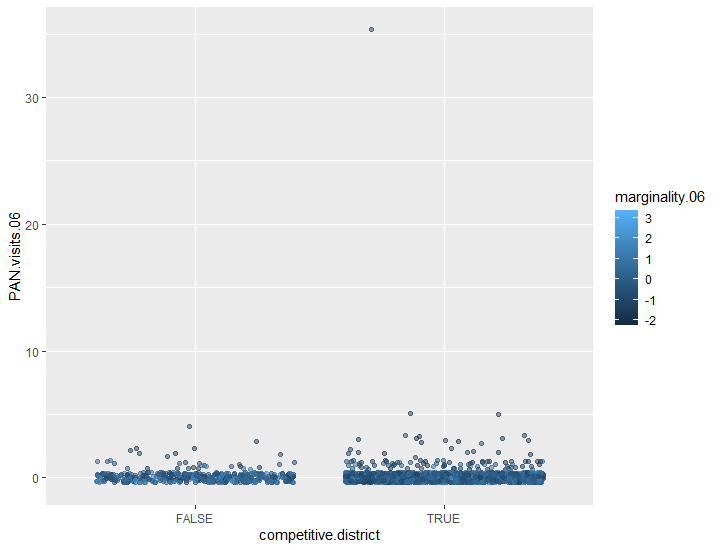
\includegraphics[scale=.80]{Visits to Competitive Districts.png}


	\item [(b)]
	Interpret the \texttt{marginality.06} and \texttt{PAN.governor.06} coefficients.

 
For all other factors being held constant, a one-unit increase in marginality is associted with a decrease of state visits by a factor of .125 (exp(-2.0814). The P value indicates it is a highly 
significant predictor of State Visits. 

For all other factors being held constant, a one-unit increase in PAN.governor.06 is associated with a decrease in the expected number of state visits by a factor of .732 (exp(-.3116)). The p value indicates it is not a highly significant predictor of state visits.
	
	\item [(c)]
	Provide the estimated mean number of visits from the winning PAN presidential candidate for a hypothetical district that was competitive (\texttt{competitive.district}=1), had an average poverty level (\texttt{marginality.06} = 0), and a PAN governor (\texttt{PAN.governor.06}=1).

 \begin{verbatim}
     pred <- data.frame(competitive.district = TRUE,
                   marginality.06 = 0,
                   PAN.governor.06 = TRUE)

predict(poisson1, newdata = pred, type = "response")
 \end{verbatim}

 Mean number of visits = 0.015 
\end{enumerate}

\includegraphics[scale=.80]{Fitted Values- Competitive District.png}

\end{document}
